\documentclass[a4paper, 11pt]{book}
\usepackage{/home/nicolas/Documents/Enseignement/Prepa/bpep/fichiers_utiles/preambule}
\newcommand{\qed}{\tag*{$\blacksquare$}}

\newcommand{\dsNB}{18}
\makeatletter
\renewcommand{\@chapapp}{Kh\^olles MPSI3 -- semaine \dsNB}
\makeatother

% \toggletrue{corrige}  % décommenter pour passer en mode corrigé

% IMPORTS automatiques
\newcommand{\f}[2]{{
		\mathchoice
		{\dfrac{#1}{#2}}
		{\dfrac{#1}{#2}}
		{\frac{#1}{#2}}
		{\frac{#1}{#2}}
}}

\newcommand{\e}[1]{{}_{\text{#1}}}
\renewcommand{\a}[0]{\alpha}
\newcommand{\w}[0]{\omega}

\usepackage{physics}

 % fin des IMPORTS automatiques

\begin{document}

\chapter{Sujet 1\siCorrige{\!\!-- corrig\'e}}
\section{Question de cours}

Définir la force de \textsc{Lorentz}~; comparer les ordres de grandeurs des
forces électriques et magnétiques au poids~; déterminer la puissance de la force
de \textsc{Lorentz} et discuter des conséquences. Démontrer qu'elle est
conservative et déterminer l'expression de l'énergie potentielle associée.

\resetQ
\subimport{/home/nicolas/Documents/Enseignement/Prepa/bpep/exercices/Colle/ressort_poids/}{sujet.tex}

\chapter{Sujet 2\siCorrige{\!\!-- corrig\'e}}
\section{Question de cours}

Savoir discuter le mouvement d'une particule en comparant son profil d'énergie
potentielle et son énergie mécanique~; état lié ou de diffusion. Expliquer
l'obtention des positions d'équilibre et leur stabilité sur un graphique
$\Ec_p(x)$. Traduire l'équilibre et sa stabilité en terme de conditions sur la
dérivée première et seconde de l'énergie potentielle.

\resetQ
\section{Chute sur corde en escalade}
On étudie une grimpeuse qui chute. Une corde d'escalade de longueur $L_0$ peut,
en première approximation, être modélisée par un ressort de longueur à vide
$L_0$ et de raideur $k = \a/L_0$, avec $\a$ une caractéristique de la corde.

\begin{center}
    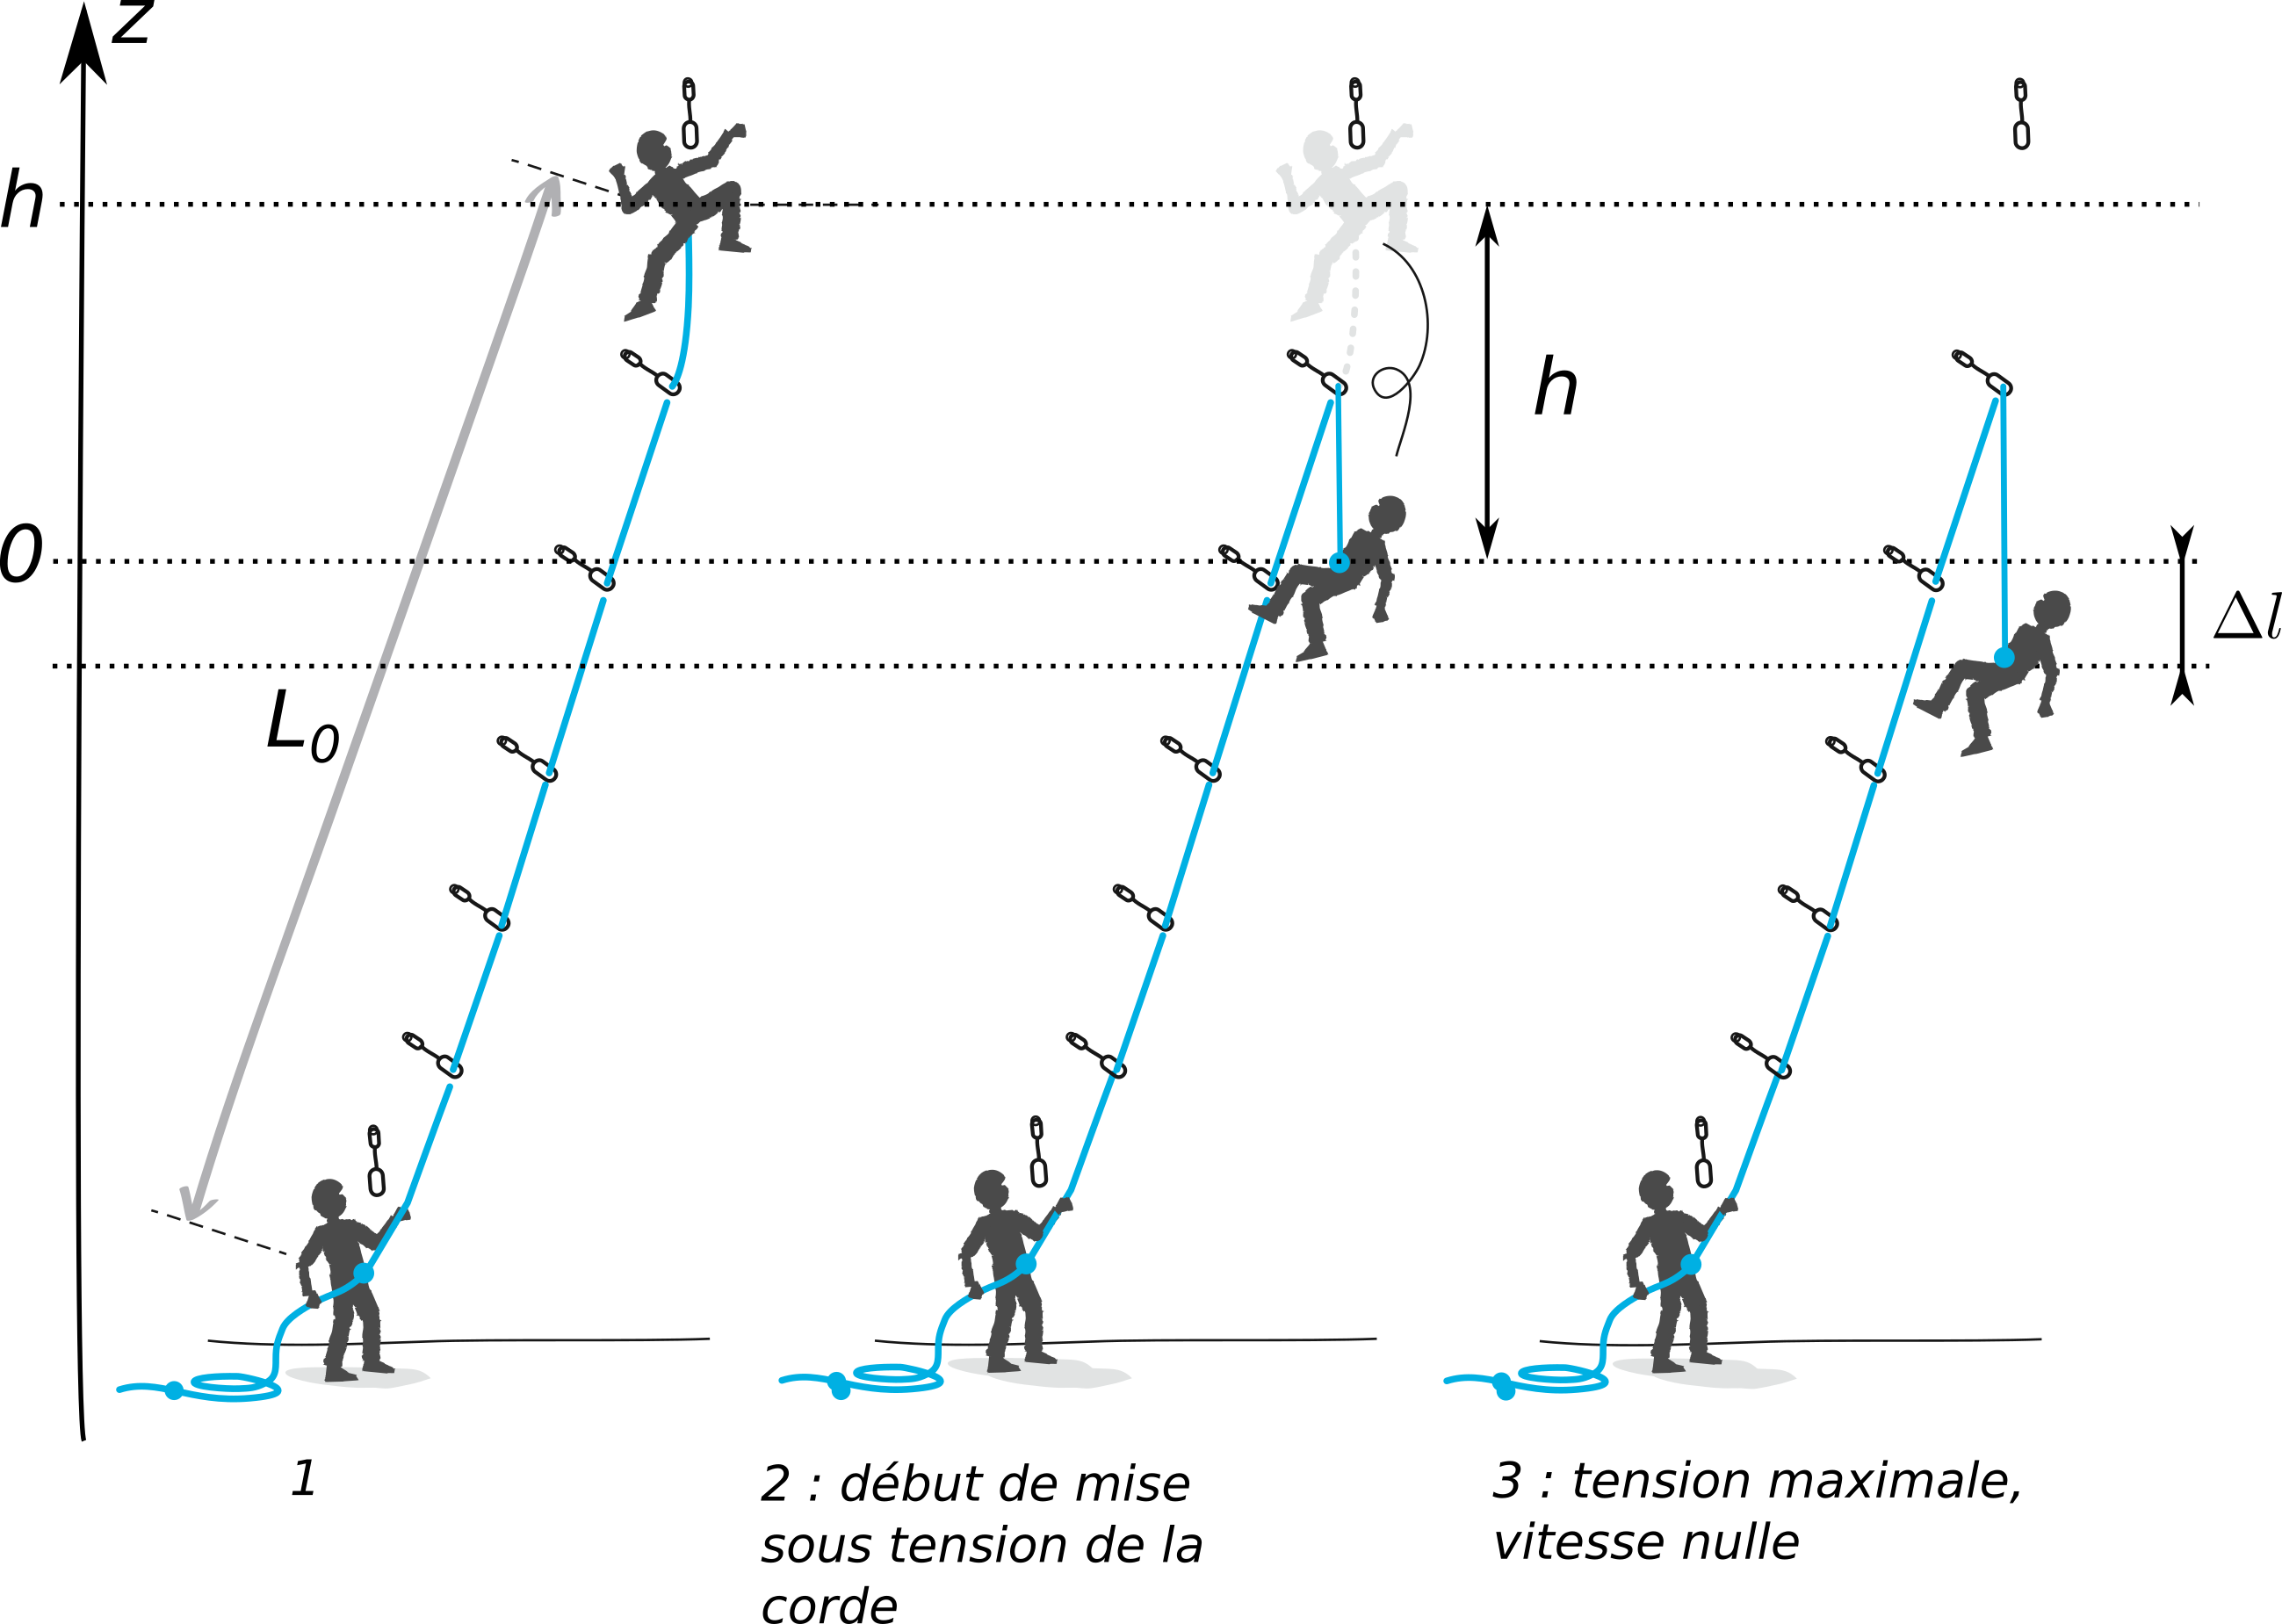
\includegraphics[width=.7\linewidth]{../../figures/ch18/chute_escalade-plain}
\end{center}

La grimpeuse est en chute libre sur une hauteur $h$ pendant laquelle la corde
n'est pas sous tension. La corde passe ensuite sous tension, et la chute se
poursuit sur une hauteur $\D l$. La vitesse de la grimpeuse devient ainsi nulle
au bout d'une hauteur totale de chute $h+\D l$.

On prendra $g = \SI{10}{m.s^{-2}}$, $\a = \SI{5.0e4}{N}$ et une grimpeuse de
masse $m = \SI{50}{kg}$. \bigbreak

\QR{À l'aide d'un bilan énergétique, donner l'expression de la vitesse
    maximale atteinte par la grimpeuse. Faire l'application numérique pour
une hauteur de chute $h = \SI{5}{m}$.}
{Pendant la chute libre, la grimpeuse ne subit que l'action du poids,
    qui est conservatif. On peut donc utiliser le TEM, avec~:
    \begin{itemize}[label=$\diamond$]
        \litem{Au début de la chute libre~:} $z = h$, $v=0 \Ra \Ec_{p,p} = mgh$ et
            $\Ec_c = 0$
        \litem{À la fin de la chute libre~:} $z = 0$, $v=v \Ra \Ec_{p,p} = 0$ et
            $\Ec_c = mv^2/2$.
    \end{itemize}
    D'où
    \begin{gather*}
        \frac{1}{2}mv^2 = mgh
        \Lra
        \boxed{v = \sqrt{2gh}}
        \qavec
        \left\{
            \begin{array}{rcl}
                g & = & \SI{10}{m.s^{-2}}\\
                h & = & \SI{5}{m}
            \end{array}
        \right.\\
        \AN
        \boxed{v = \SI{10}{m.s^{-1}}}
    \end{gather*}
}
\QR{Toujours à l'aide d'une méthode énergétique, donner l'expression de
    l'allongement maximal $\D l$ de la corde. On supposera $\D l \ll h$ afin
de simplifier le calcul.}
{On peut utiliser le TEM entre le point tout en haut et le point le
    plus bas, ou entre le point O et le point le plus bas. Faisons le
    premier cas~:
    \begin{itemize}[label=$\diamond$]
        \litem{Au début de la chute libre~:} $z = h$, $v=0 \Ra \Ec_{p,p} = mgh$ et
            $\Ec_c = 0$
        \litem{À la fin de la chute amortie~:} $z = -\D l$, $v=0 \Ra \Ec_{p,p}
            = -mg\D l$, \fbox{$\Ec_{p,el} = k\D l^2/2$} et $\Ec_c = 0$.
    \end{itemize}
    Ainsi,
    \begin{gather*}
        mgh = \frac{1}{2}k\D l^2 + mg(-\D l)
        \Lra
        mg(h+\underbracket[1pt]{\cancel{\D l}}_{\ll h}) = \frac{1}{2}k\D l^2
        \Lra
        \boxed{\D l = \sqrt{\frac{2mgh}{k}}}
        \qed
    \end{gather*}
    La solution trouvée est plausible~: homogène, augmente avec $m$, $h$ et
    $g$ mais diminue avec $k$.
}
\QR{Donner enfin l'expression de la norme de la force maximal $F_{\max}$
    qu'exerce la corde sur la grimpeuse. On introduira le facteur de chute
$f = h/L_0$.}
{En norme, une force de rappel s'exprime $F = k(\ell -\ell_0)$, soit
    ici
    \begin{gather*}
        F_{\max} = k\D l = \sqrt{2mgh\,k} = \sqrt{2mgh\frac{\a}{L_0}}
        \\\Lra
        \boxed{F_{\max} = \sqrt{2mg\a f}}
        \qed
    \end{gather*}
}
\QR{Au-delà d'une force de \SI{12}{kN}, les dommages sur le corps humain
    deviennent importants. Que vaut $F_{\max}$ pour une chute de $h =
\SI{4}{m}$ sur une corde de longueur $L_0 = \SI{4}{m}$~? Conclure.}
{On fait l'application numérique~:
    \begin{gather*}
        \qavec
        \left\{
            \begin{array}{rcl}
                m & = & \SI{50}{kg}\\
                g & = & \SI{10}{m.s^{-2}}\\
                \a & = & \SI{5.0e4}{N}\\
                f & = & \num{1}
            \end{array}
        \right.\\
        \AN
        \boxed{F_{\max} = \SI{10}{kN}}
    \end{gather*}
    Il n'y a donc pas de risque aggravé pour la grimpeuse avec cette chute.
}
\QR{Une chute d'un mètre arrêtée par une corde de \SI{50}{cm} est-elle
    plus ou moins dangereuse qu'une chute de \SI{4}{m} arrêtée par une corde
de \SI{8}{m}~?}
{Dans le premier cas, $f_1 = 2$~; dans le second, $f_2 = \num{0.5}$. Or,
$F_{\max}$ évolue en $\sqrt{f}$, donc plus $f$ augmente plus la force
subie augmente~: le premier cas est donc 2 fois plus dangereux que le
premier~!
}

\chapter{Sujet 3\siCorrige{\!\!-- corrig\'e}}
\section{Question de cours}

Action de $\Bf$ uniforme sur une particule chargée avec $\vfo\perp\Bf$~:
présenter la situation, et prouver que le mouvement est uniforme, plan et
circulaire. On déterminera l'équation de la trajectoire en introduisant le rayon
et la pulsation cyclotron, ainsi que les équations scalaires.

\resetQ
\section{Positions d'équilibre d'un anneau sur un cercle}
\begin{minipage}{0.60\linewidth}
    Un anneau assimilable à un point matériel M de masse $m$ peut glisser sans
    frottement sur une glissière circulaire de rayon $R$ et de centre O.
    L'anneau est attaché à un ressort de raideur $k$ dont une extrémité est
    fixée à la glissière au point A. Sa position est repérée par l'angle $\tt$
    entre le rayon OM et l'axe horizontal (O$x$). Pour simplifier les calculs,
    on considérera que la longueur à vide $\ell_0$ du ressort est nulle.
\end{minipage}
\hfill
\begin{minipage}{0.35\linewidth}
    \begin{center}
        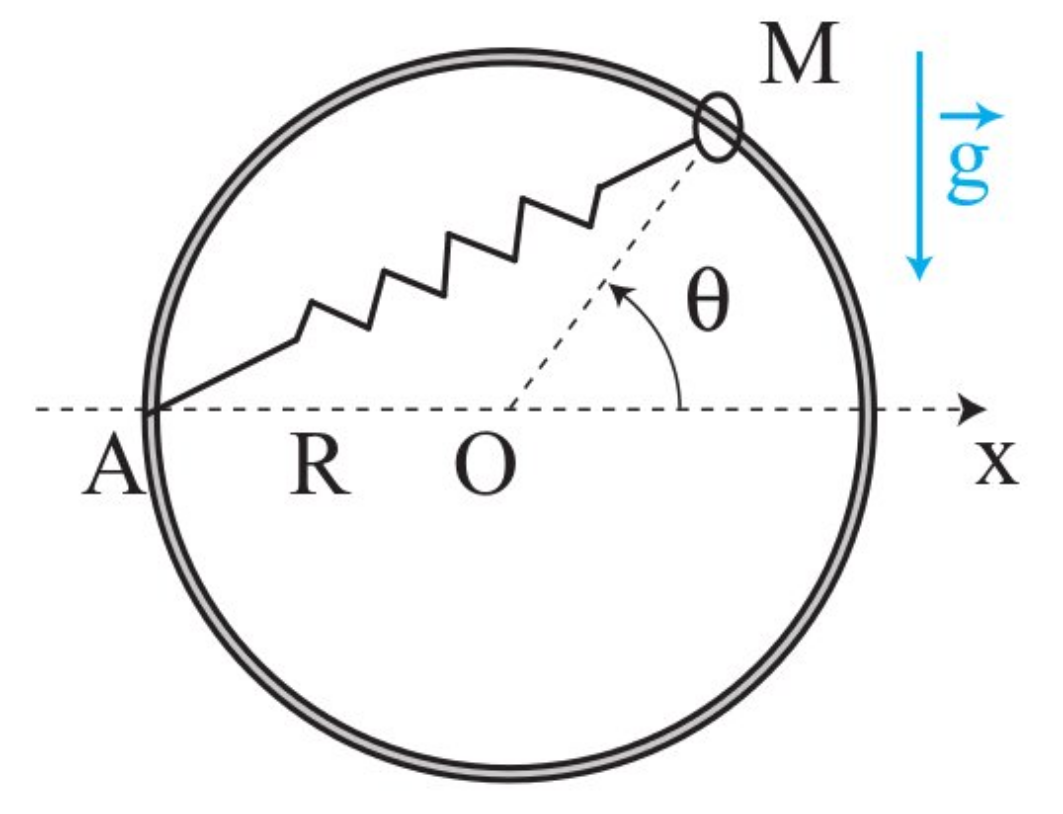
\includegraphics[width=.9\linewidth]{../../figures/ch18/anneau_cercle_ressort-plain}
    \end{center}
\end{minipage}

\QR{Montrer que la longueur $\ell$ s'exprime $\ell =
R\sqrt{2(1+\cos\tt)}$.}
{
    \begin{minipage}[t]{0.25\linewidth}
        ~
        \begin{center}
            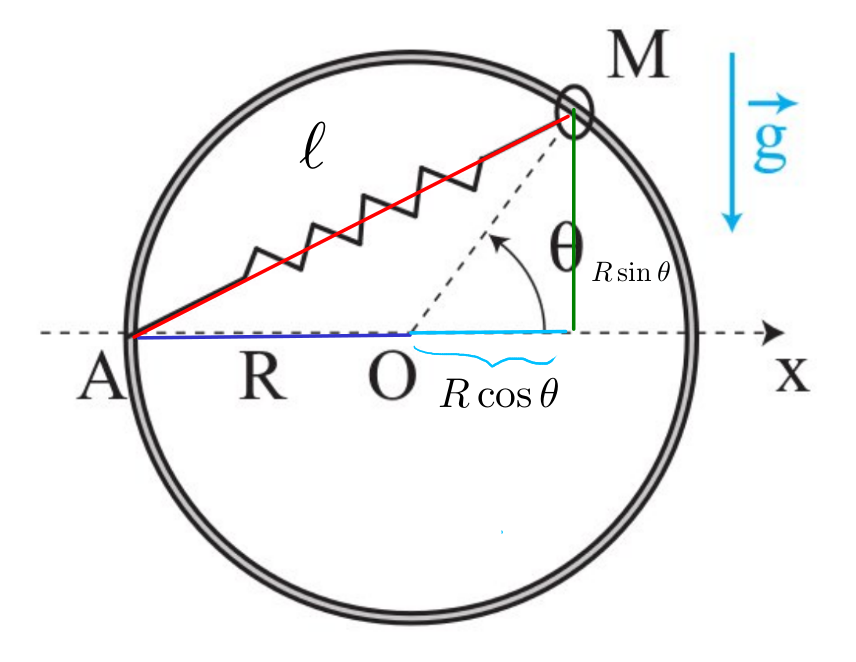
\includegraphics[width=\linewidth]{../../figures/ch18/anneau_cercle_ressort-proj}
            \captionsetup{justification=centering}
            \captionof{figure}{Détermination de $\ell$}
            \label{fig:anncercproj}
        \end{center}
    \end{minipage}
    \hfill
    \begin{minipage}[t]{0.70\linewidth}
        On peut réutiliser la relation de \textsc{Chasles} pour écrire
        $\vv{\rm AM} = \vv{\rm AO} + \OM$ et déterminer la distance en prenant
        la norme, mais ici une simple utilisation du théorème de
        \textsc{Pythagore} suffit. On projette M sur l'axe $x$ pour avoir
        \begin{align*}
            \ell^2 &= (R+R\cos\tt)^2 + (R\sin\tt)^2
            \\\Lra
            \ell^2 &= R^2 + 2R^2\cos\tt + R^2(\cos^2\tt + \sin^2\tt)
            \\\Lra
            \ell^2 &= 2R^2(1+\cos\tt)
            \\\Lra
            \Aboxed{\ell &= R\sqrt{2(1+\cos\tt)}}
            \qed
        \end{align*}
    \end{minipage}
}
\QR{Exprimer l'énergie potentielle $\Ec_p$ du système constitué de
l'anneau et du ressort en fonction de l'angle $\tt$.}
{L'énergie potentielle totale $\Ec_p$ est constituée de l'énergie
    potentielle de pesanteur de l'anneau et de l'énergie potentielle
    élastique du ressort. Pour $\Ec_{p,p}$ avec origine en O, on a une
    altitude $R\sin\tt$~; pour $\Ec_{p,el}$ on a la différence de longueur à
    a vide $\ell -\ell_0$ avec $\ell_0 = 0$, d'où
    \begin{align*}
        \Ec_p &= \Ec_{p,p} + \Ec_{p,el}
        \\\Lra
        \Ec_p &= mgR\sin\tt + \frac{k}{2}\ell^2
        \\\Lra
        \Aboxed{\Ec_p &= mgR\sin\tt + kR^2(1+\cos\tt)}
        \qed
    \end{align*}
}
\QR{Déterminer les positions d'équilibre de l'anneau.}
{On trouve les positions d'équilibre de l'anneau en trouvant les angles
    $\tt_{\req}$ tels que la dérivée de $\Ec_p$ s'annule, soit
    \begin{align*}
        \eval{\dv{\Ec_p}{\tt}}_{\tt_{\req}} &= -kR^2\sin\tt_{\req} +
        mgR\cos\tt_{\req} = 0
        \\\Lra
        \sin\tt_{\req} &= \frac{mg\cancel{R}}{kR^{\cancel{2}}}\cos\tt_{\req}
        \\\Lra
        \tan\tt_{\req} &= \frac{mg}{kR}
        \\\Lra
        \boxed{\tt_{\req,1} = \arctan(\frac{mg}{kR})}
        \quad&\text{et}\quad
        \boxed{\tt_{\req,2} = \pi + \arctan(\frac{mg}{kR})}
        \qed
    \end{align*}
    avec $\tt_{\req,1}$ compris entre 0 et \ang{90}, et $\tt_{\req,2}$ compris
    entre 180 et \ang{270}.
}
\QR{Préciser si les positions d'équilibre obtenues sont stables.}
{On étudie la stabilité des positions en évaluant la dérivée seconde de
    $\Ec_p$ en ce point et en vérifiant son signe. On obtient
    \begin{align*}
        \eval{\dv[2]{\Ec_p}{\tt}}_{\tt_{\req}} &= -kR^2\cos\tt_{\req}
        -mgR\sin\tt_{\req}
        \\\Lra
        \eval{\dv[2]{\Ec_p}{\tt}}_{\tt_{\req}} &= -\left(kR^2 +
            \frac{m^2g^2}{k}\right)\cos\tt_{\req}
    \end{align*}
    en utilisant les résultats précédents sur la dérivée première de
    $\Ec_p$. L'intérieur de la parenthèse étant positif, le signe de cette
    dérivée seconde est opposé à celui du cosinus de la position
    d'équilibre. Or,
    $\cos\tt_{\req,1} > 0$ et $\cos\tt_{\req,2} < 0$, donc
    \begin{gather*}
        \boxed{\eval{\dv[2]{\Ec_p}{\tt}}_{\tt_{\req,1}} < 0}
        \qet
        \boxed{\eval{\dv[2]{\Ec_p}{\tt}}_{\tt_{\req,2}} > 0}
        \qed
    \end{gather*}
    La première position est donc instable, et la seconde stable.
    \begin{figure}[htbp]
        \centering
        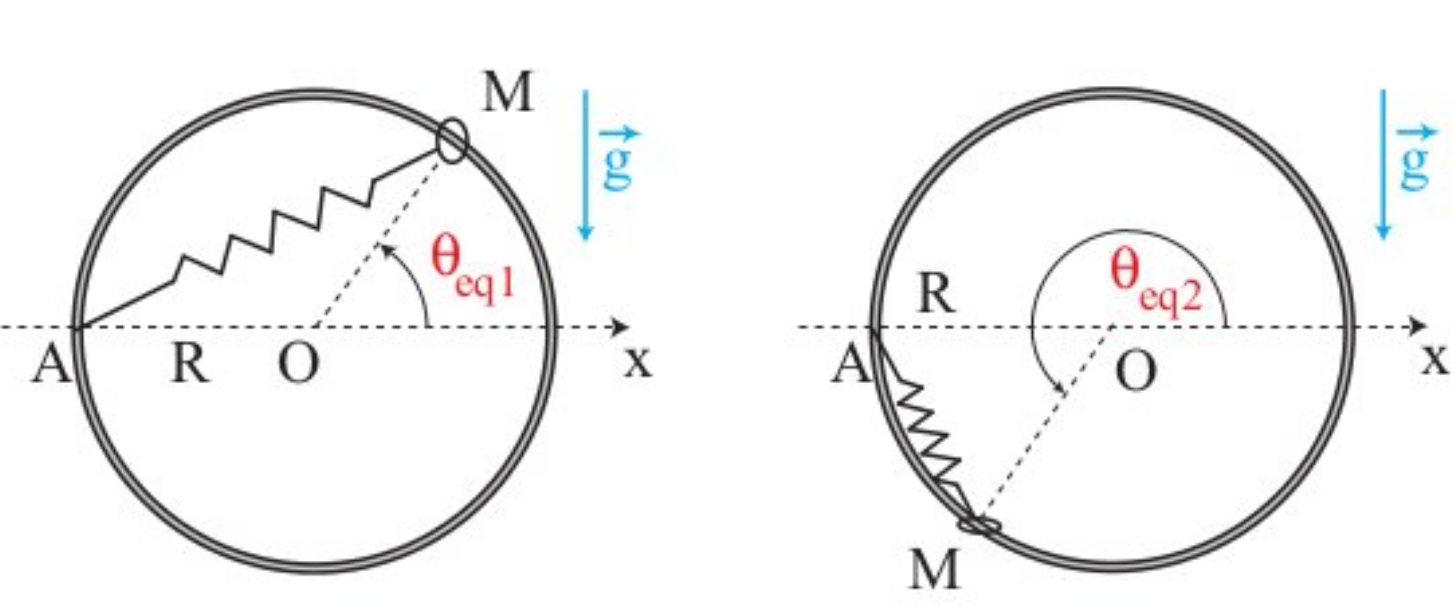
\includegraphics[width=.5\linewidth]{../../figures/ch18/anneau_cercle_ressort-corr_eq}
        \captionsetup{justification=centering}
        \caption{Positions d'équilibre du système}
        \label{fig:anncerccorr}
    \end{figure}
}

\label{LastPage}
\end{document}
